
\documentclass{beamer}
\usepackage{subcaption}
\usepackage{float}
\usepackage{graphicx}
\usefonttheme[onlymath]{serif}

\usetheme{Warsaw}

\bibliographystyle{ieeetr}
\hypersetup{pdfstartview={Fit}} 
\setbeamertemplate{footline}[frame number]
\beamersetuncovermixins{\opaqueness<1>{25}}{\opaqueness<2->{15}}
\begin{document}
	\title{Graph Analysis}

\author{Sergio Yaksic}

\date{\today}


\begin{frame}
\titlepage
\end{frame}
	

\section{Abstract}


\begin{frame}\frametitle{Abstract}

Using a python program, an statistical analysis about the connectivity patterns over scale-free graphs is presented. 
We compare our statistical results with the theoretical degree distribution $P(k)$ and degree-degree correlation function $P(k|x)$ 

\end{frame}
	

\section{Degree Distribution}


\begin{frame}\frametitle{Degree Distribution}

\begin{figure}[hbt!]
%\caption{barabasi-albert-graph(100000,3)}
\includegraphics[width=0.8\textwidth]{./temp/exp/results/Image01.eps}

\end{figure}


Here is a plot of the degree distribution of a barabasi-albert graph. The yellow squares represent the statistical probability of choosing a node of degree $k$.

\end{frame}
	

\subsection{Power law Distribution}


\begin{frame}\frametitle{Power law Distribution}
\begin{columns}
\begin{column}{6.5cm}
\begin{figure}[hbt!]
%\caption{barabasi-albert-graph(100000,3)}
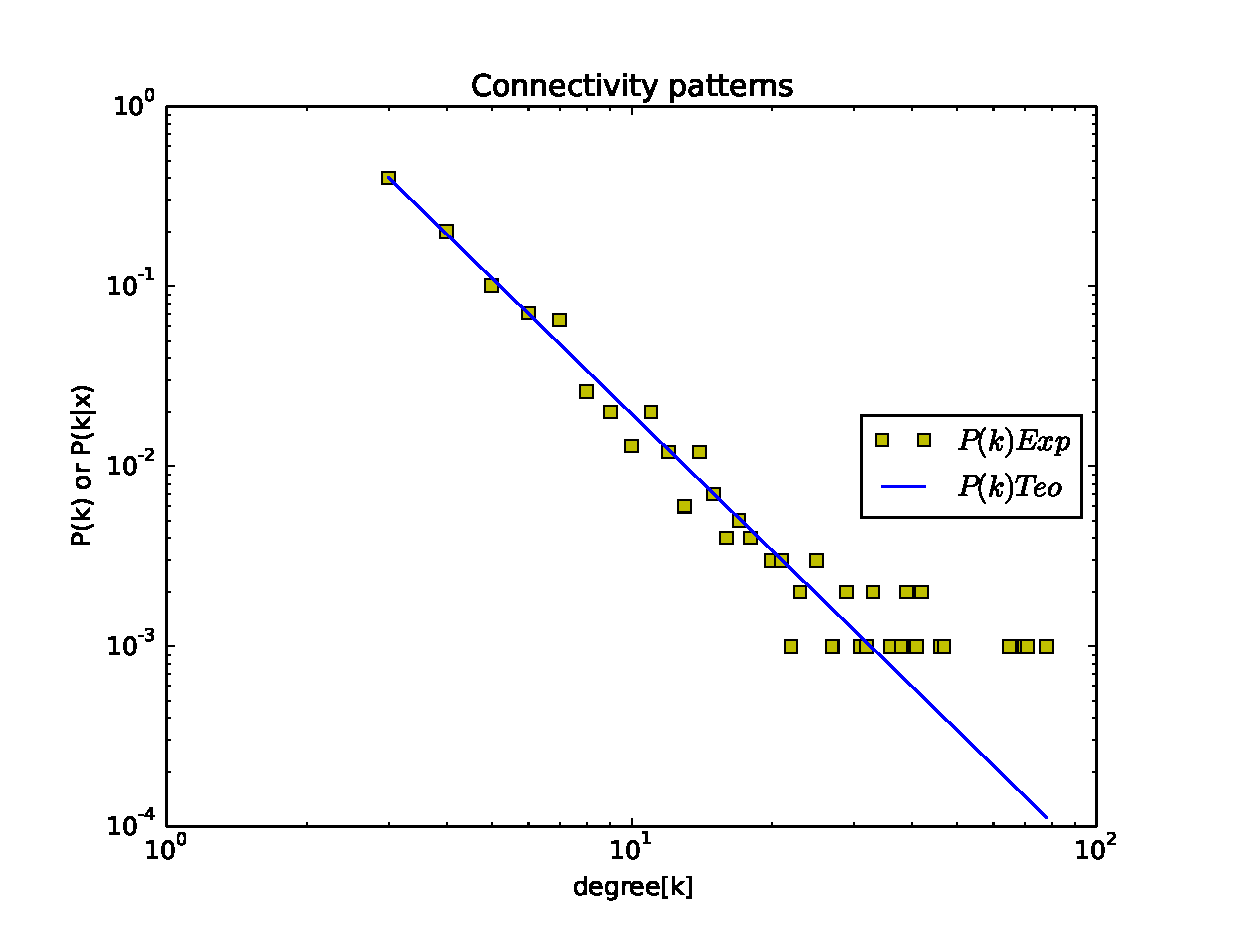
\includegraphics[width=1.0\textwidth]{./temp/exp/results/Image02.eps}

\end{figure}
\end{column}
\begin{column}{3.5cm}
\begin{equation}
\label{eq:degree_dist}
P(k)=Ck{-\gamma}
\end{equation}
\end{column}
\end{columns}


The blue line represents the best fit (the one that minimizes the sum of squared errors) for theoretical equation \ref{eq:degree_dist}.


\end{frame}
	

\section{Degree-degree correlation function}


\begin{frame}\frametitle{Degree-degree correlation function}


Using equation \ref{eq:degree-degree_correlation} presented by vespignati we plotted the degree-degree correlation function, that is the probability of choosing a node of degree $k$ connected to a node of degree $x$.


\begin{equation}
\label{eq:degree-degree_correlation}
P(k|x)=\frac{kP(k)}{\langle k \rangle}=\frac{kCk{-\gamma}}{\langle k \rangle}
\end{equation}

\end{frame}
	

\subsection{Theoretical $P(k|x)$}


\begin{frame}\frametitle{Theoretical $P(k|x)$}
Theoretical $P(k|x)$ using the parameters of blue curve $P(k)$ and $P(k|x=\langle k \rangle)$ as reference.

\begin{figure}[hbt!]
%\caption{barabasi-albert-graph(100000,3)}
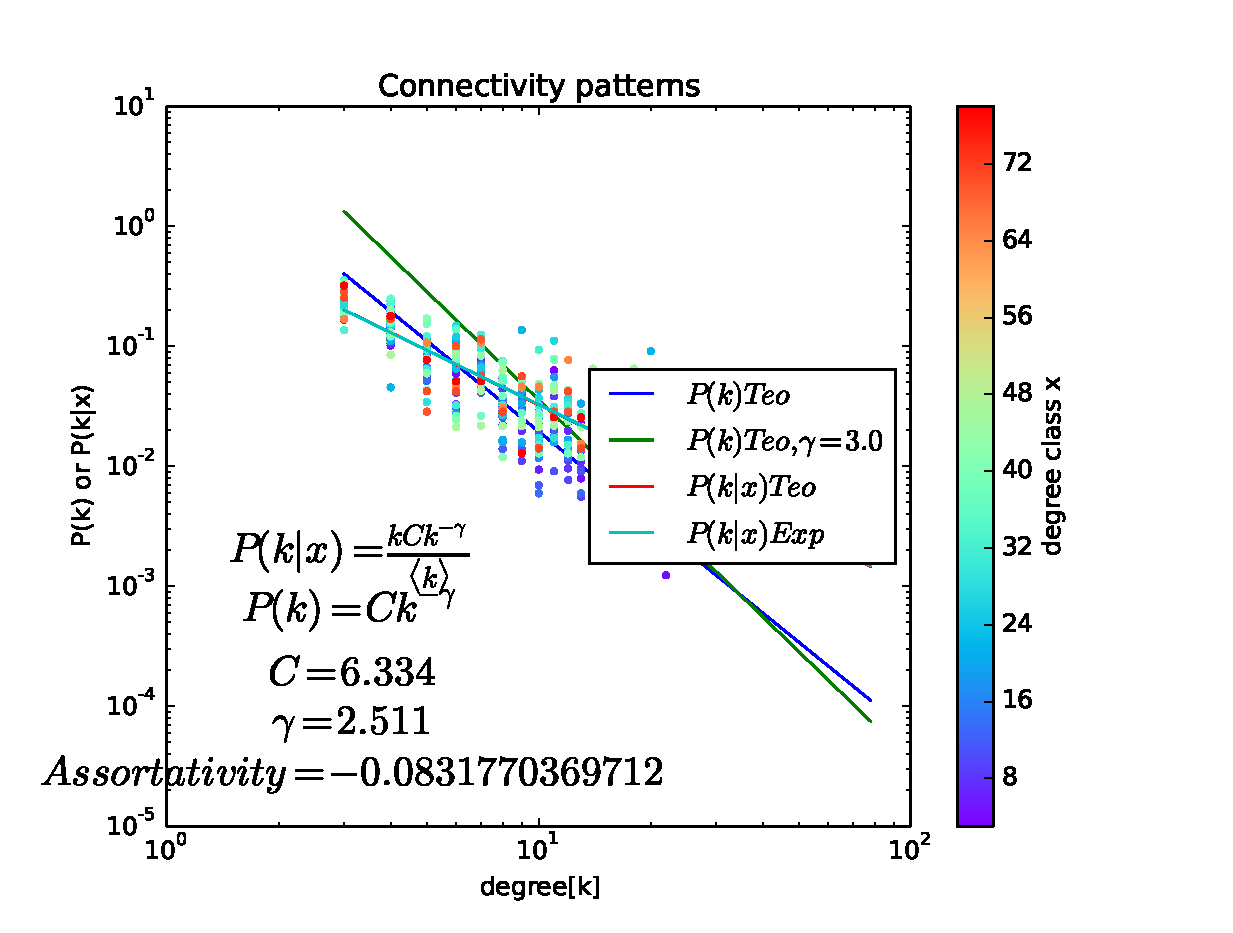
\includegraphics[width=0.8\textwidth]{./temp/exp/results/Image03.eps}

\end{figure}
\end{frame}
	

\end{document}

